\documentclass[a4paper,12pt]{article}
\usepackage[utf8]{inputenc}
\usepackage[spanish]{babel}
\usepackage{color}
\usepackage{parskip}
\usepackage{graphicx}
\usepackage{multirow}
\usepackage{listings}
\usepackage{vmargin}
\usepackage{datetime}
\newdate{date}{27}{10}{2017}
\graphicspath{ {imagenes/} }
\definecolor{mygreen}{rgb}{0,0.6,0}
\definecolor{lbcolor}{rgb}{0.9,0.9,0.9}
\usepackage{epstopdf}
\usepackage{float}


\setpapersize{A4}
\setmargins{2.5cm}       % margen izquierdo
{1.5cm}                        % margen superior
{16.5cm}                      % anchura del texto
{23.42cm}                    % altura del texto
{10pt}                           % altura de los encabezados
{1cm}                           % espacio entre el texto y los encabezados
{0pt}                             % altura del pie de página
{2cm}     

\lstset{
    tabsize=4,    
%   rulecolor=,
    language=[GNU]C++,
        basicstyle=\tiny,
        aboveskip={1.5\baselineskip},
        columns=fixed,
        showstringspaces=false,
        extendedchars=false,
        breaklines=true,
        prebreak = \raisebox{0ex}[0ex][0ex]{\ensuremath{\hookleftarrow}},
        frame=single,
        showtabs=false,
        showspaces=false,
        showstringspaces=false,
        identifierstyle=\ttfamily,
        keywordstyle=\color[rgb]{0,0,1},
        commentstyle=\color[rgb]{0.026,0.112,0.095},
        stringstyle=\color{red},
        numberstyle=\color[rgb]{0.205, 0.142, 0.73},
%        \lstdefinestyle{C++}{language=C++,style=numbers}’.
}


\begin{document}
\title{Práctica de Laboratorio 2}
\author{
Christofer Fabián Chávez Carazas \\
\small{Universidad Nacional de San Agustín de Arequipa} \\
\small{Escuela Profesional de Ciencia de la Computación} \\
\small{Computación Gráfica}
}
\date{\displaydate{date}}

\maketitle

\begin{enumerate}
 \item \textbf{Compile y ejecute el siguiente código}

\begin{figure}[H]
 \centering
 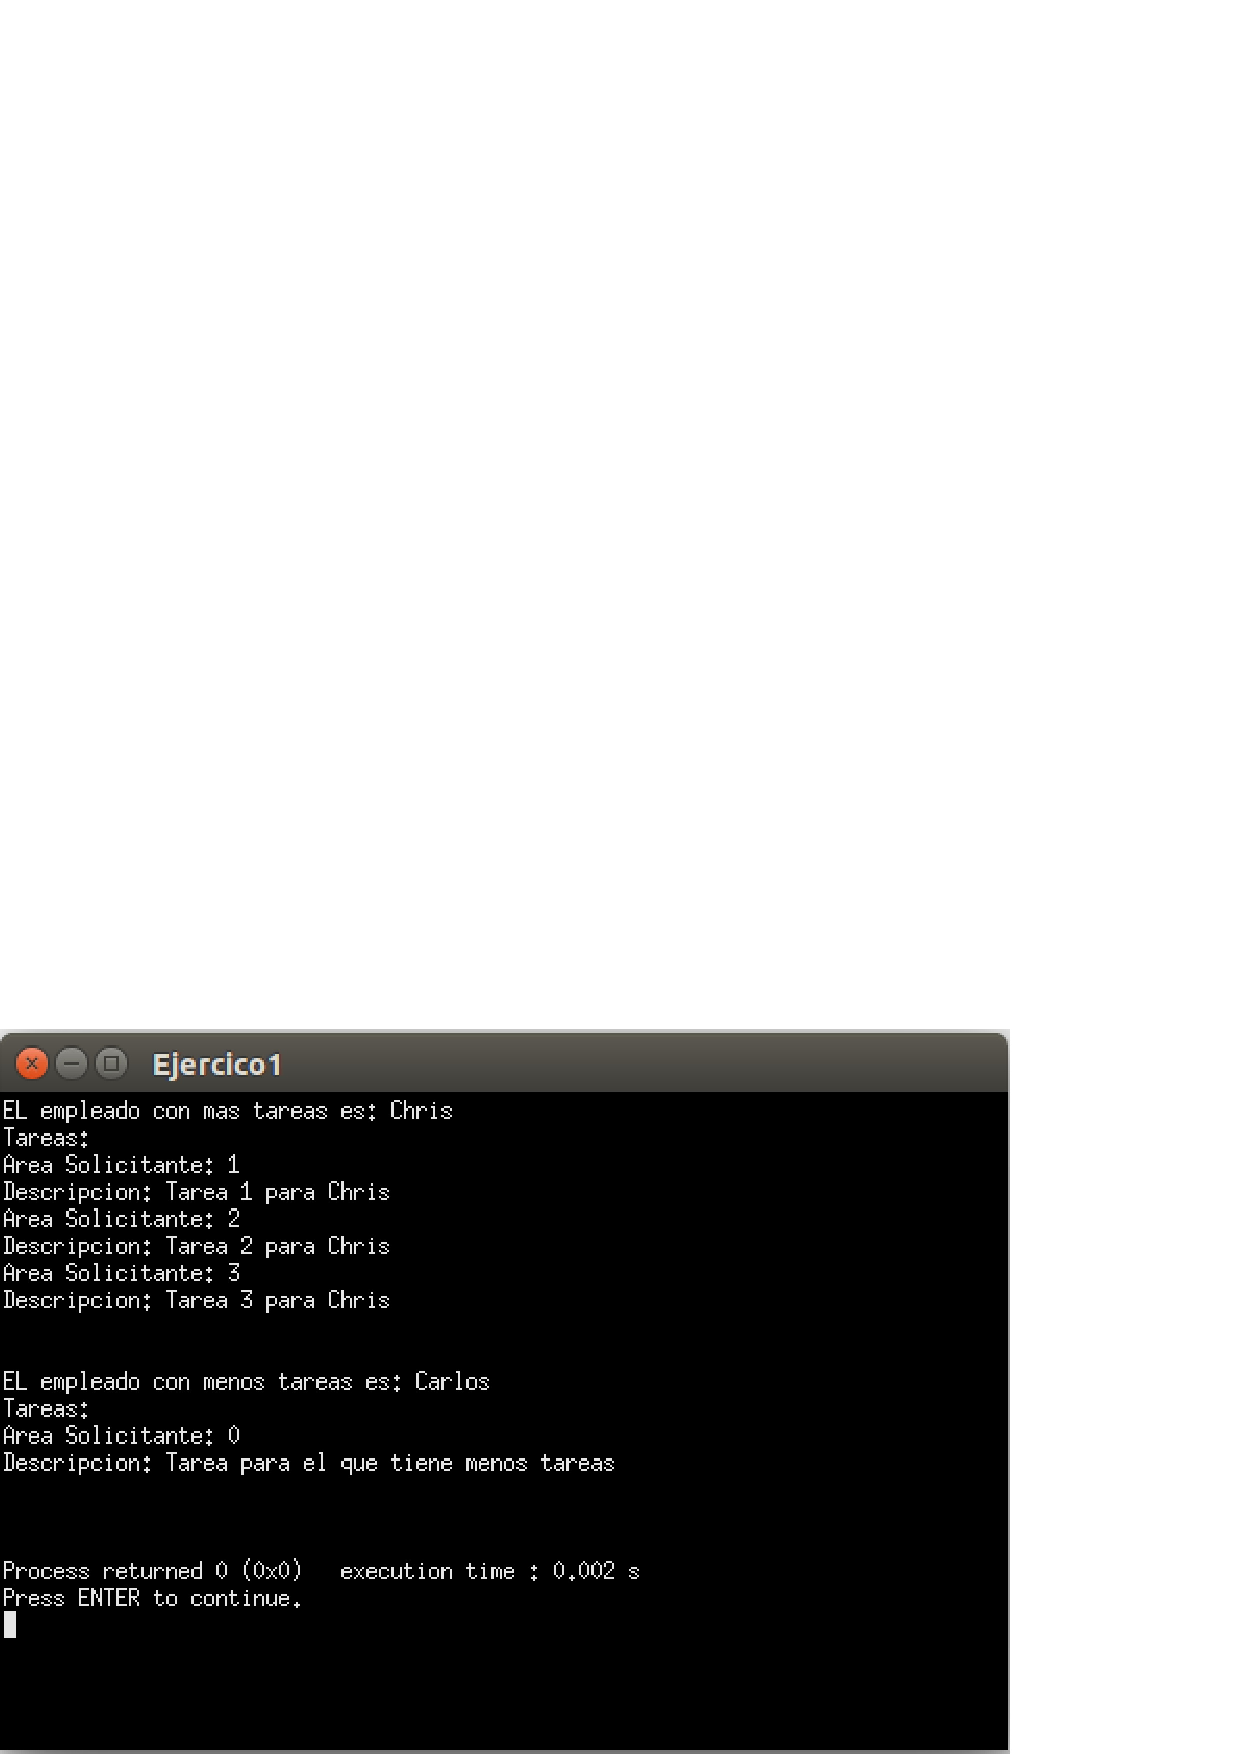
\includegraphics[scale = 0.5]{1.png}
 \caption{Resultados}
\end{figure}

 \item \textbf{Explique qué función cumple cada línea de código}
 
 \begin{lstlisting}
    glBegin(GL_LINE_STRIP);
        for(k = 0; k < 12; k++){
            glVertex2i(x + k*50, dataValue[k]);
        }
    glEnd();  
 \end{lstlisting}
 En esta parte del código se dibujan las líneas del gráfico. El punto x es el punto de referencia dado al inicio más un desplazamiento. El punto y
 es el valor del dato actual.
 
 \begin{lstlisting}
    for(k = 0; k < 12; k++){
        glRasterPos2i(xRaster + k*50,dataValue[k] - 4);
        glutBitmapCharacter (GLUT_BITMAP_9_BY_15,'*');
    }
 \end{lstlisting}
 En esta parte del código se dibujan los asteriscos que indican los valores de la función. Igual que el anterior, el punto x es el punto de referencia dado antes más un
 desplazamiento, El punto x es el valor del dato actual más un desplazamiento, para que quede bien alineado con la función.
 
 \begin{lstlisting}
    for(month = 0; month < 12; month++){
        glRasterPos2i(xRaster,yRaster);
        for(k = 3*month; k < 3*month + 3; k++){
            glutBitmapCharacter(GLUT_BITMAP_HELVETICA_12,label[k]);
        }
        xRaster += 50;
    }
 \end{lstlisting}
 En esta parte del código se escribe la leyenda de cada valor. Cada leyenda cuenta con 3 caracteres que están guardados en una lista.
 
\item \textbf{Cambie la función \textit{lineGraph} por el de \textit{barChart}, luego compile el programa}

\begin{figure}[H]
 \centering
 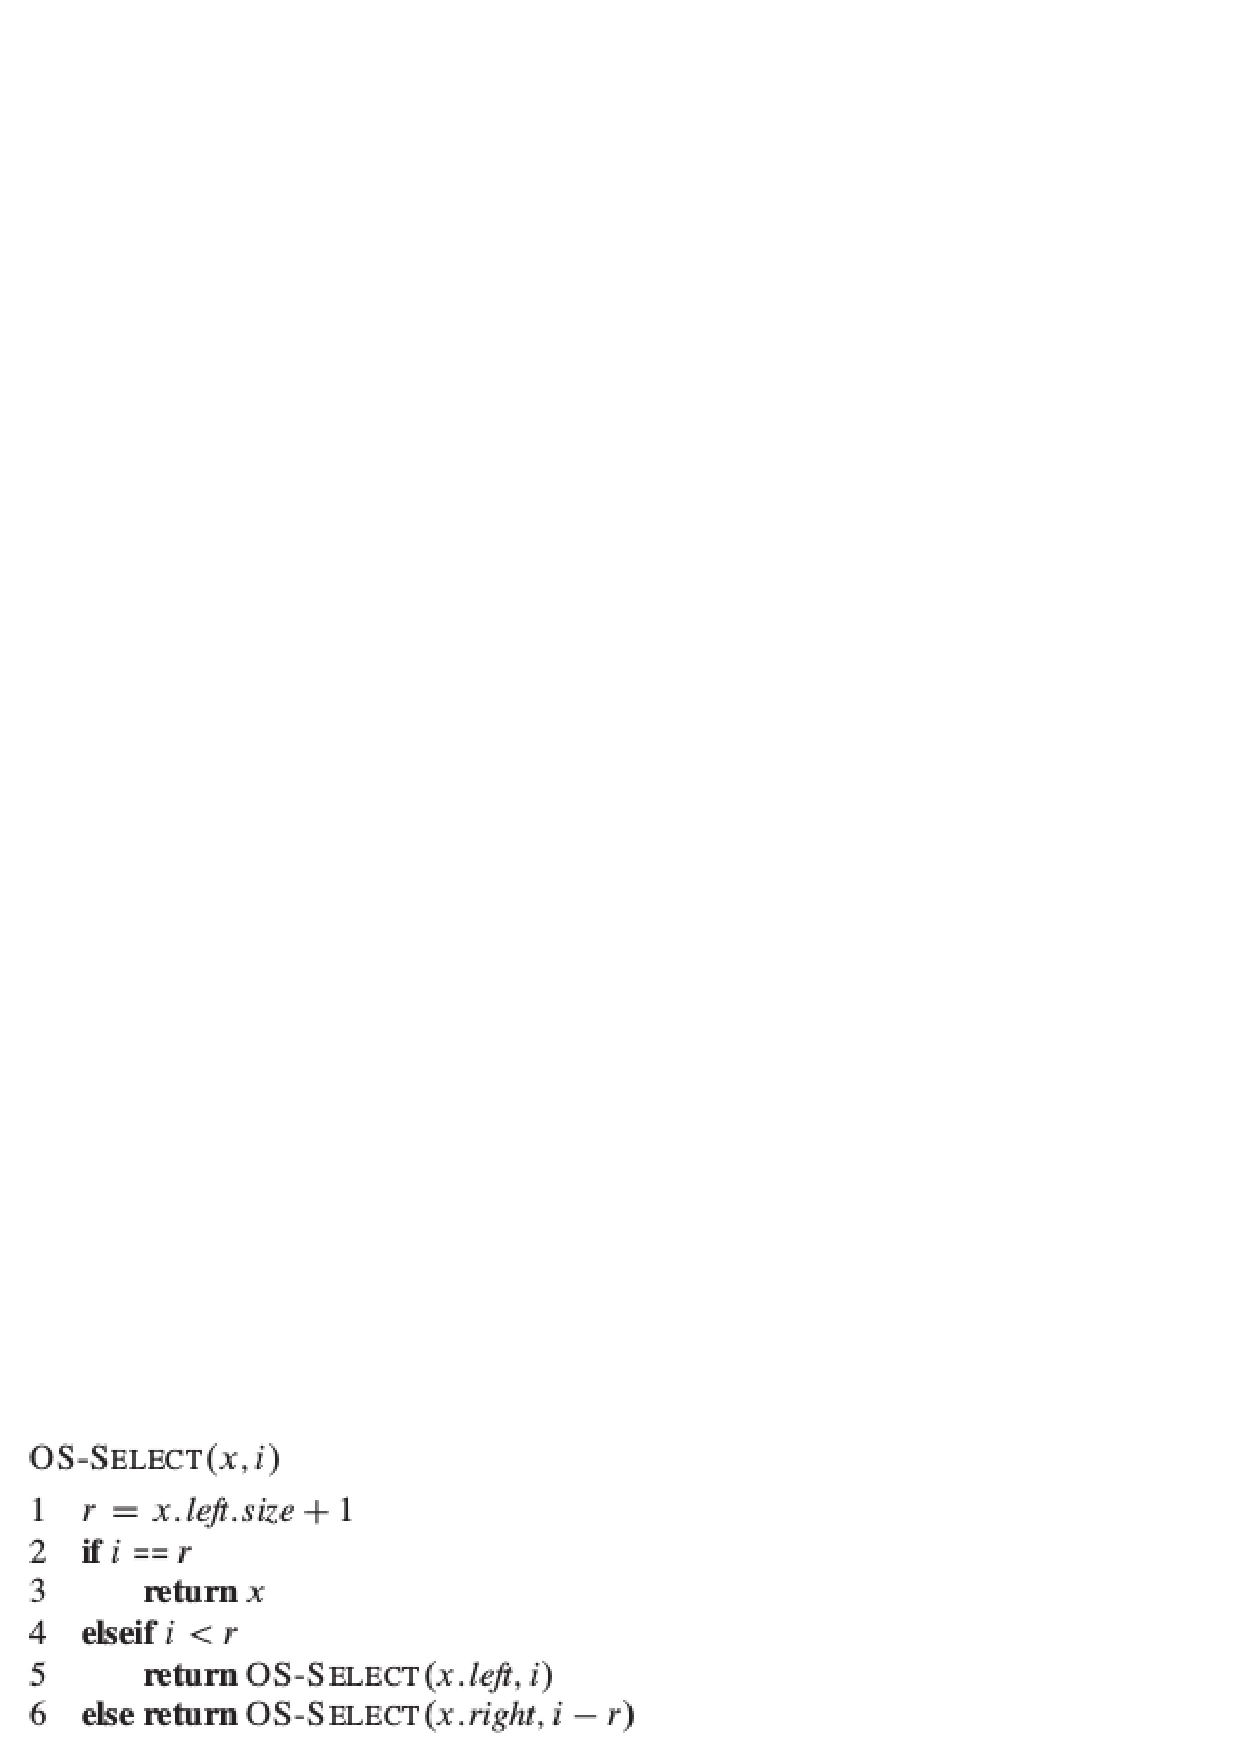
\includegraphics[scale = 0.5]{2.png}
 \caption{Resultados}
\end{figure}


\item \textbf{Construya un programa donde se muestre, en líneas y en barras, las ventanas de un producto en los últimos seis meses del año. EL gráfico debe ser parecido
a la siguiente figura. Debe ser posible agregar una línea de tendencia.}

El código es una combinación de los dos anteriores.

\begin{lstlisting}
#include <GL/glut.h>

GLsizei winWidth = 600, winHeight = 500;
GLint xRaster = 25, yRaster = 150;
int months = 6;
GLubyte label[18] = {'J','u','l','A','u','g','S','e','p',
'O','c','t','N','o','v','D','e','c'};
GLint dataValue[6] = {180,190,220,250,330,450};

void init(void){
	glClearColor(1.0,1.0,1.0,1.0);
	glMatrixMode(GL_PROJECTION);
	gluOrtho2D(0.0, 600.0, 0.0, 500.0);
}

void bartChart(void){
	GLint month, k;

	glClear(GL_COLOR_BUFFER_BIT);

	glColor3f(1.0,0.0,0.0);
	for(k = 0; k < months; k++){
		glRecti(20 + k * 50, 165, 40 + k * 50, dataValue[k]);
	}
	glColor3f(0.0, 0.0, 0.0);
	xRaster = 20;
	for(month = 0; month < months; month++){
		glRasterPos2i(xRaster,yRaster);
		for(k = 3*month; k < 3*month + 3; k++){
			glutBitmapCharacter(GLUT_BITMAP_HELVETICA_12,label[k]);
		}
		xRaster += 50;
	}


	GLint x = 30;
    glColor3f(0.0, 0.0,1.0);
    glBegin(GL_LINE_STRIP);
        for(k = 0; k < months; k++){
            glVertex2i(x + k*50, dataValue[k]);
        }
    glEnd();
	xRaster = 25;
    for(k = 0; k < months; k++){
        glRasterPos2i(xRaster + k*50,dataValue[k] - 4);
        glutBitmapCharacter (GLUT_BITMAP_9_BY_15,'*');
    }
    glFlush();
	
}

int main(int argc, char **argv){
	glutInit(&argc, argv);
	glutInitDisplayMode(GLUT_SINGLE | GLUT_RGB);
	glutInitWindowPosition(100, 100);
	glutInitWindowSize(winWidth, winHeight);
	glutCreateWindow("Line Chart Data Plor");

	init();
	glutDisplayFunc(bartChart);

	glutMainLoop();
	return 0;
}
\end{lstlisting}

\begin{figure}[H]
 \centering
 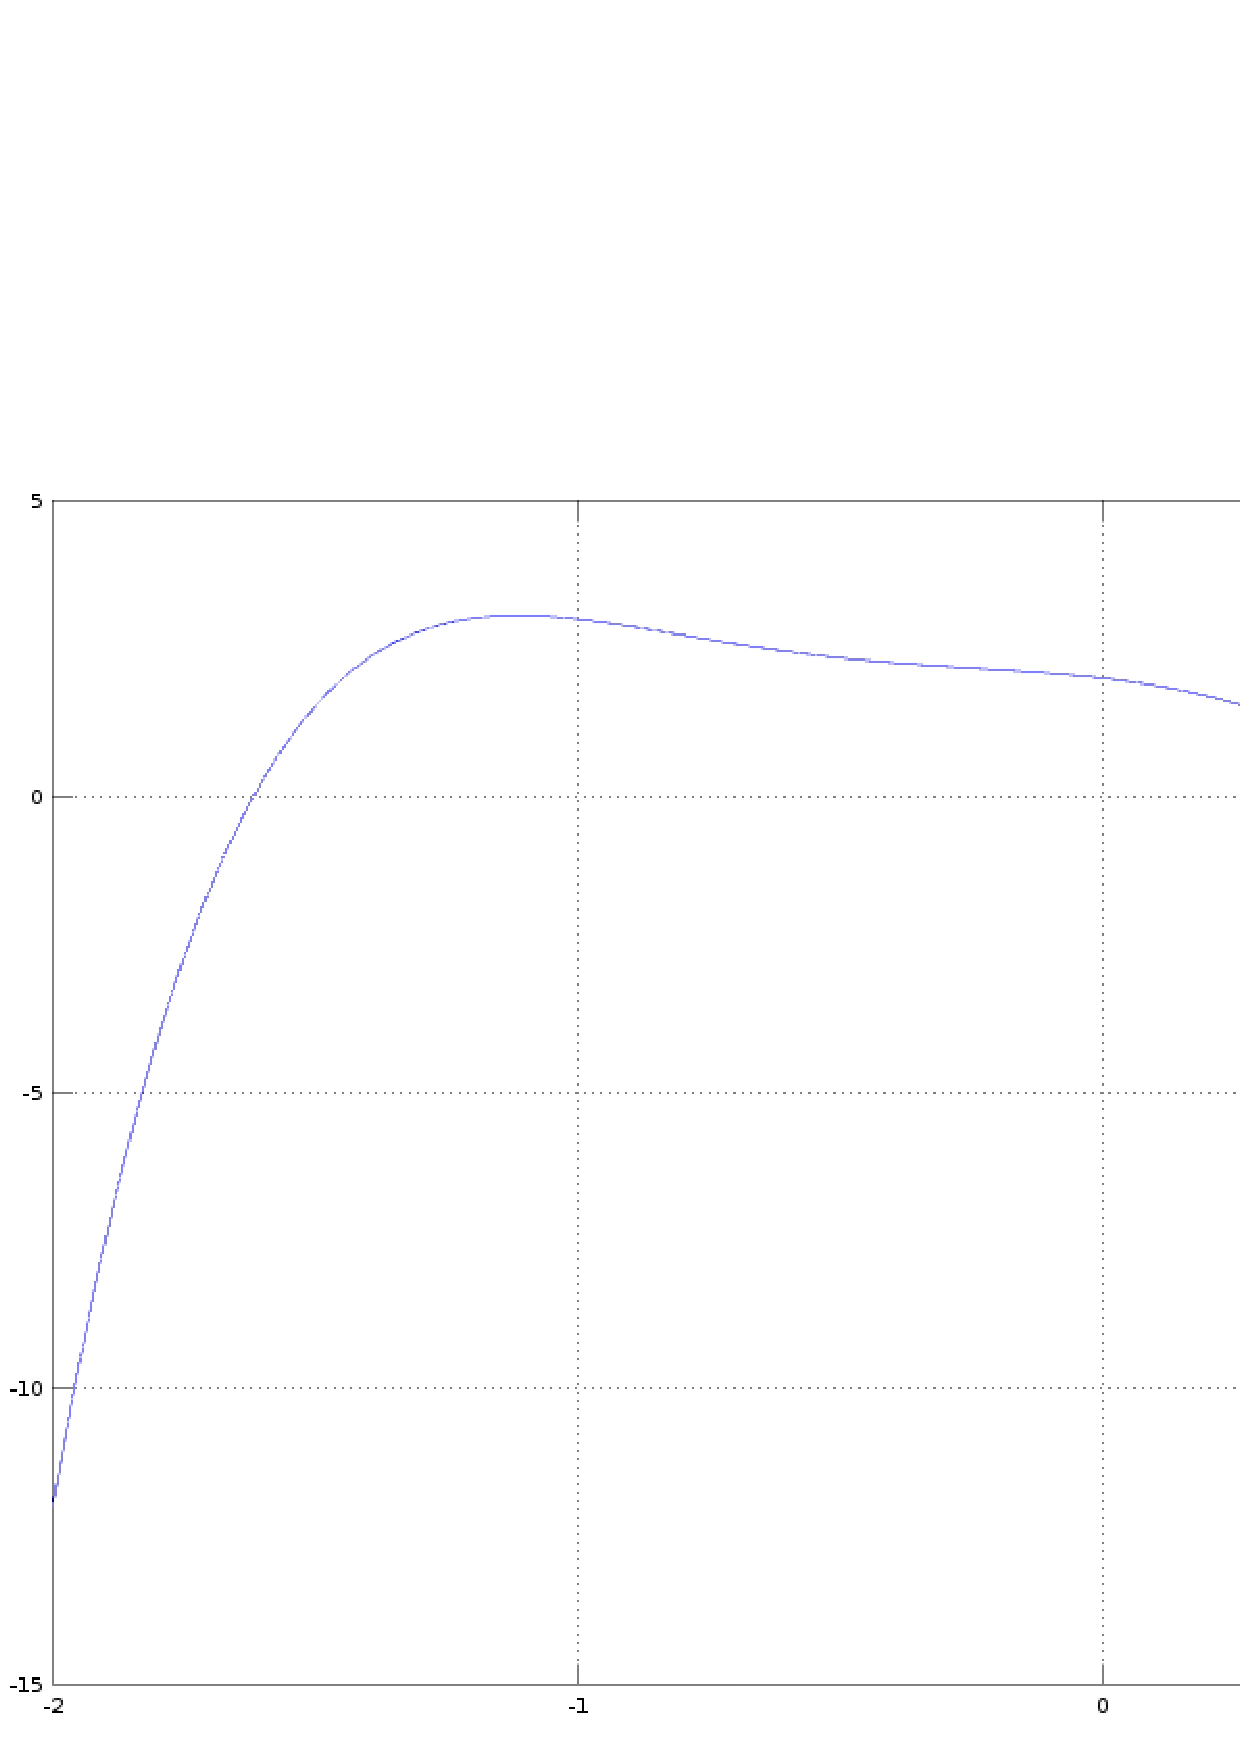
\includegraphics[scale = 0.5]{3.png}
 \caption{Resultados}
\end{figure}

\item \textbf{El siguiente programa construye una figura circular, utilizando la rutina del punto medio para generar el circulo.}

\begin{figure}[H]
 \centering
 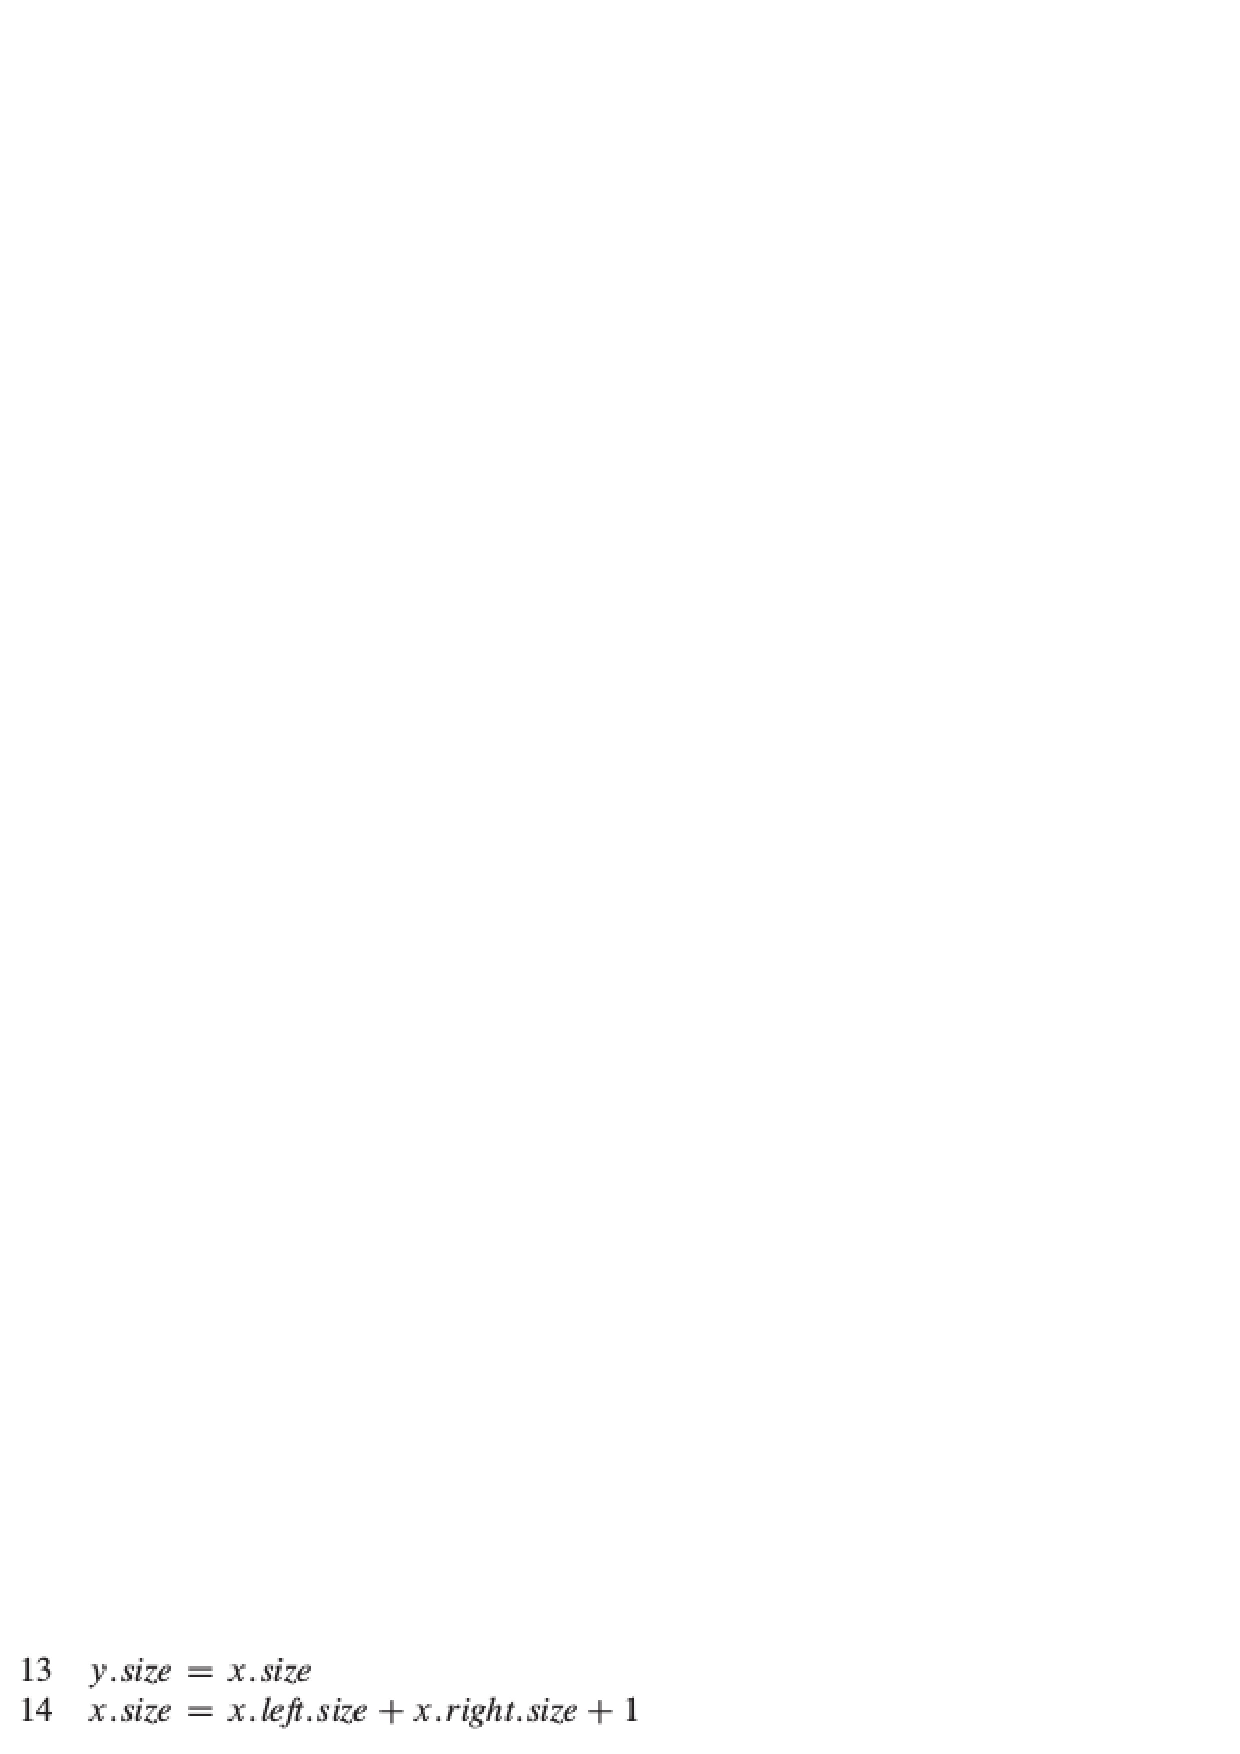
\includegraphics[scale = 0.5]{4.png}
 \caption{Resultados}
\end{figure}

\item \textbf{Las gráficas de sectores circulares se utilizan para mostrar la contribución porcentual de una serie de partes individuales a un todo.
Modifique el programa anterior para construir una gráfica de sectores circulares, el resultado debe ser parecido a la siguiente figura.}

La única función modificada del código anterior es \textit{pieChart}. Se van acumulando los valores para sacar
el siguiente ángulo. Con ese ángulo se saca el seno y el coseno para hallar el punto del circulo donde terminará
la línea.

\begin{lstlisting}
void pieChart(void){
    srcPt circCtr, piePt;
    GLint radius = winWidth / 4;
    GLdouble sliceAngle, previousSliceAngle = 0.0;
    GLint k, nSlices = 12;
    GLfloat dataValues[12] = {10.0,7.0,13.0,5.0,13.0,14.0,3.0,16.0,5.0,3.0,17.0,8.0};
    GLfloat total = 0.0;
    GLfloat dataSum = 0.0;
    srcPt secondPoint;
    circCtr.x = winWidth / 2;
    circCtr.y = winHeight / 2;
    for(int i = 0; i < nSlices; i++){
        total += dataValues[i];
    }
    for(int i = 0; i < nSlices; i++){
        dataSum += dataValues[i];
        sliceAngle = getAngle(dataSum, total);
        secondPoint.x = circCtr.x + cos(sliceAngle * PI/180) * radius;
        secondPoint.y = circCtr.y + sin(sliceAngle * PI/180) * radius;
        drawLine(circCtr,secondPoint);
    }
    circleMidPoint(circCtr, radius);
}
\end{lstlisting}

\begin{figure}[H]
 \centering
 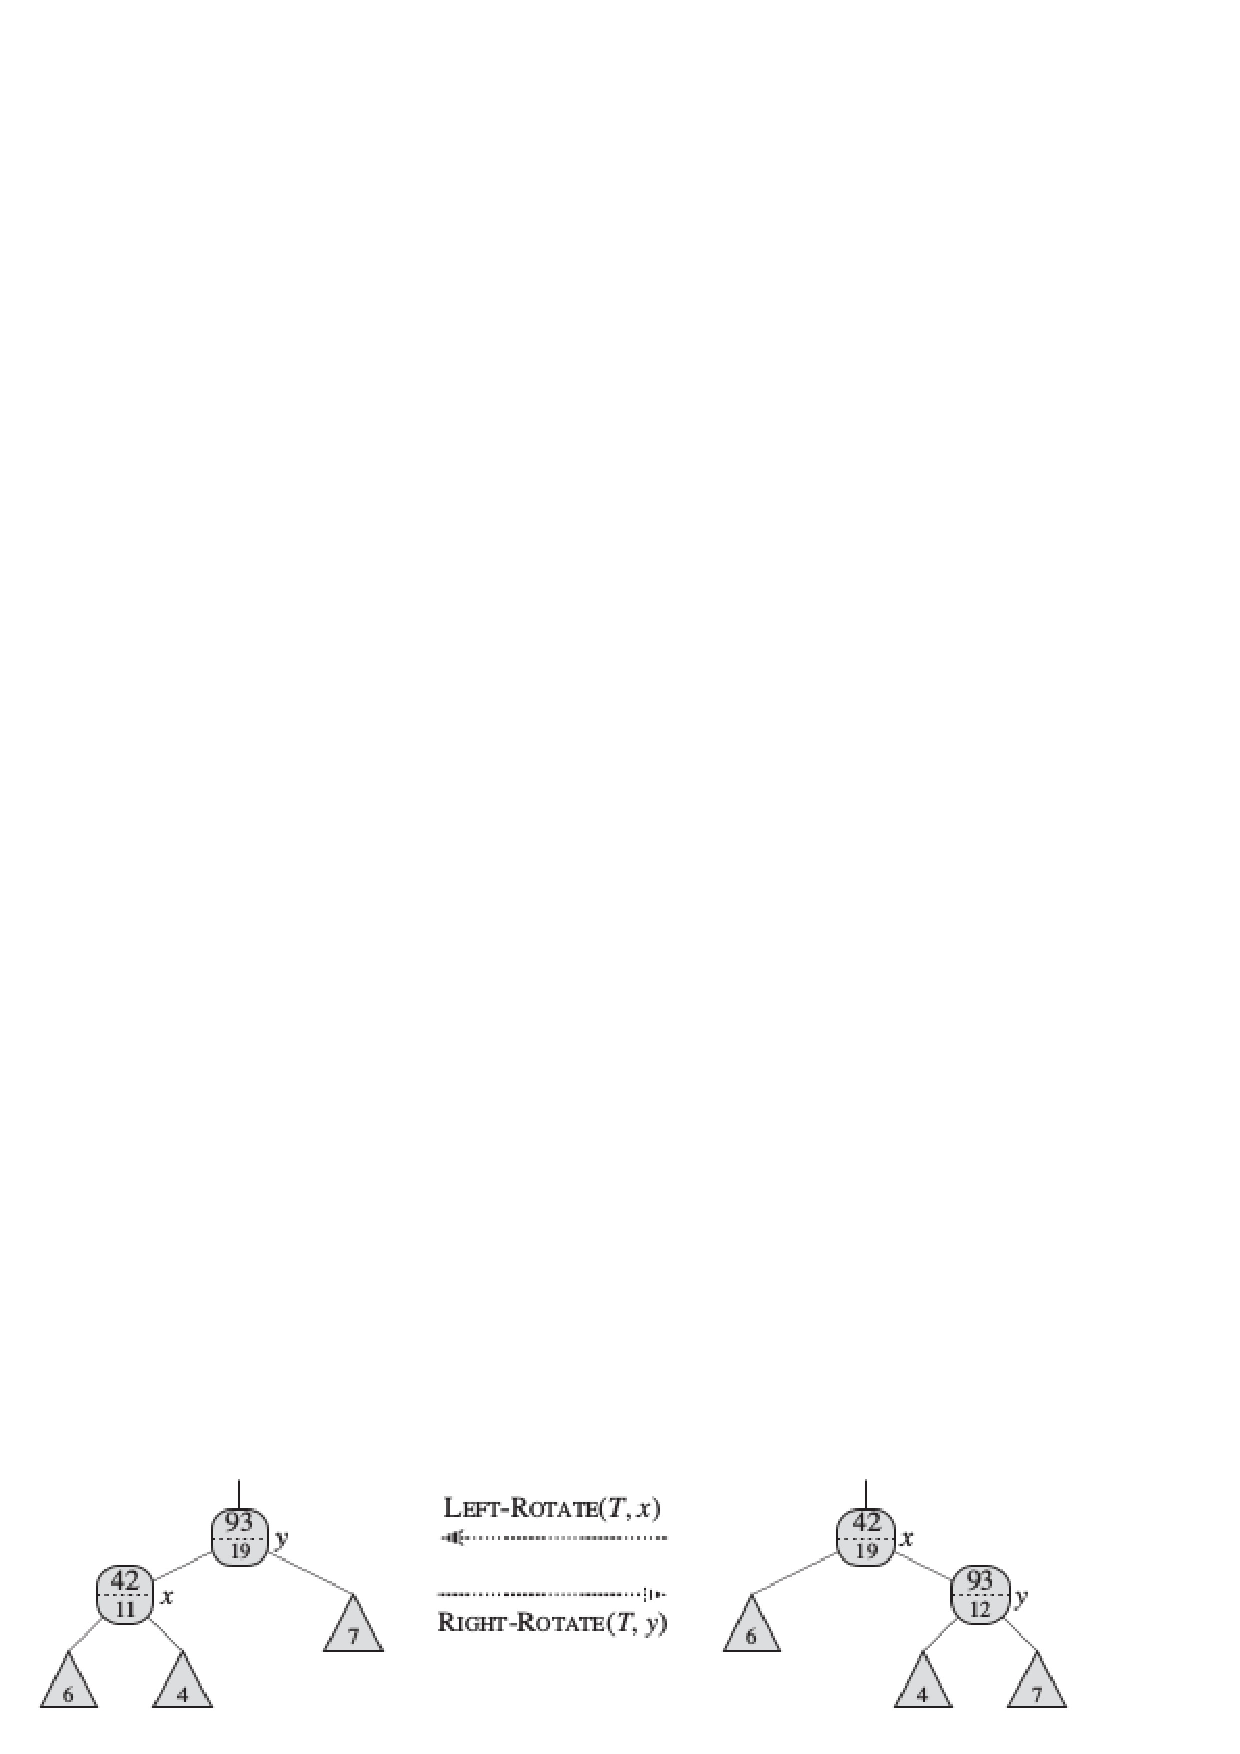
\includegraphics[scale = 0.5]{5.png}
 \caption{Resultados}
\end{figure}




 
\end{enumerate}
\end{document}

